% !TEX program = xelatex
\documentclass[10pt,letterpaper,twocolumn]{article}

\usepackage[top=0.75in, bottom=0.75in, left=0.75in, right=0.75in]{geometry}
\usepackage{fontspec}
\usepackage{unicode-math}
\setmainfont{Latin Modern Roman}[
  Extension=.otf,
  UprightFont=lmroman10-regular,
  BoldFont=lmroman10-bold,
  ItalicFont=lmroman10-italic,
  BoldItalicFont=lmroman10-bolditalic,
]
\setsansfont{Latin Modern Sans}[
  Extension=.otf,
  UprightFont=lmsans10-regular,
  BoldFont=lmsans10-bold,
  ItalicFont=lmsans10-oblique,
  BoldItalicFont=lmsans10-boldoblique,
]
\newfontfamily\acbold{ywft-processing-bold}[Path=../../system/public/type/webfonts/,Extension=.ttf]
\setmonofont{Latin Modern Mono}[
  Extension=.otf,
  UprightFont=lmmono10-regular,
  ItalicFont=lmmono10-italic,
  Scale=0.85,
]

\usepackage{xcolor}
\usepackage{titlesec}
\usepackage{enumitem}
\usepackage{booktabs}
\usepackage{tabularx}
\usepackage{fancyhdr}
\usepackage{hyperref}
\usepackage{xurl}
\usepackage{graphicx}
\graphicspath{{figures/}{../arxiv-ac/figures/}}
\usepackage{ragged2e}
\usepackage{microtype}
\usepackage{natbib}
\usepackage{tikz}
\usetikzlibrary{positioning,arrows.meta,fit}
\usepackage{../ac-source-bundle}
\usepackage{balance}

\definecolor{acpink}{RGB}{180,72,135}
\definecolor{acpurple}{RGB}{120,80,180}
\definecolor{acdark}{RGB}{64,56,74}
\definecolor{acgray}{RGB}{119,119,119}

\hypersetup{colorlinks=true,linkcolor=acpurple,urlcolor=acpurple,citecolor=acpurple,
  pdftitle={Edit the Harness, Not the Model},
  pdfauthor={@jeffrey}}

\titleformat{\section}{\normalfont\bfseries\normalsize\uppercase}{\thesection.}{0.5em}{}
\titlespacing{\section}{0pt}{1.2em}{0.3em}
\titleformat{\subsection}{\normalfont\bfseries\small}{\thesubsection}{0.5em}{}
\titlespacing{\subsection}{0pt}{0.8em}{0.2em}

\newcommand{\acdot}{{\color{acpink}.}}
\newcommand{\ac}{Aesthetic{\acdot}Computer}

\pagestyle{fancy}\fancyhf{}
\renewcommand{\headrulewidth}{0pt}
\fancyhead[C]{\footnotesize\color{acpink}\textit{Field report --- \ac{} papers}}
\fancyfoot[C]{\footnotesize\thepage}

\newcommand{\code}[1]{\texttt{#1}}
\renewcommand{\dbltopfraction}{0.8}
\setcounter{dbltopnumber}{2}
% Latin Modern has no check mark; draw one.
\newcommand{\yes}{\tikz[baseline=-0.15ex]\draw[acpink,line width=0.9pt,line cap=round,line join=round] (0,0.45ex)--(0.32ex,0.05ex)--(0.95ex,0.95ex);}

\setlist[itemize]{nosep, leftmargin=1.2em, itemsep=0.1em}
\setlist[enumerate]{nosep, leftmargin=1.4em, itemsep=0.1em}
\setlength{\columnsep}{1.8em}
\setlength{\parindent}{1em}
\setlength{\parskip}{0.3em}

\tolerance=800
\emergencystretch=1em
\hyphenpenalty=50

\begin{document}

\twocolumn[{%
\begin{center}

\includegraphics[height=4em]{pals}\par\vspace{0.5em}
{\acbold\fontsize{21pt}{25pt}\selectfont\color{acdark} Edit the Harness, Not the Model}\par
\vspace{0.45em}
{\normalfont\itshape\fontsize{11pt}{13pt}\selectfont\color{acpink} Carrying Harness$^2$ over to Aesel, a piece-writing agent, in one day}\par
\vspace{0.3em}
{\normalfont\fontsize{9pt}{11pt}\selectfont\color{acgray} Seven rounds, two models, three adopted edits, and what a single run per arm cannot tell you.}\par
\vspace{0.6em}
{\normalsize\href{https://prompt.ac/@jeffrey}{@jeffrey}}\par
{\small\color{acgray} \ac{} --- October 18, 2026}\par
{\small\color{acgray} ORCID: \href{https://orcid.org/0009-0007-4460-4913}{0009-0007-4460-4913}}\par
\vspace{0.3em}
{\small\color{acpurple} \url{https://aesthetic.computer}}\par
\vspace{0.6em}
\rule{\textwidth}{1.5pt}
\vspace{0.5em}
\end{center}

\begin{quote}
\small\noindent\textbf{Abstract.}
Harness$^2$ \citep{xu2026harness2} improves an agent without touching its
weights: for each task it runs the current harness, has two editors propose
changes from the run's transcript, re-runs the task under each change, composes
the edits whose runs did better, and keeps a library of what each edit did. We
carried the method over to Aesel, \ac{}'s harness for writing pieces, in one
day. The prompt text moved into named markdown sections that compile
byte-identically into every surface (verified across 1,536 terminal states and
290 bridge and native states). A headless runner plays every save in a browser
and returns what breaks to the model before its write completes. A
refinement loop drives both, with the Claude CLI as editor, composer, blind
selector and reflector. Seven live rounds on three interaction tasks, two with
the default hosted model and one with Claude Sonnet~5.5 writing the pieces,
produced three adopted edits and three lessons for the library. The default model
benefited; Sonnet~5.5 delivered every task in two or three rounds and rarely
needed the help. Every finding rests on one run per arm, and we say so.
\end{quote}
\vspace{1em}
}]

\section{Introduction}
\label{sec:intro}

A \emph{harness} is everything around a model that lets it act: the system
prompt, guardrails, tool guidance, memory, skills and the loop that carries
tool results back. When an agent writes a bad piece, the usual remedies are a
better model or a better prompt written by hand after reading a complaint.
Harness$^2$ proposes a third: make the harness itself the thing being
optimised, task by task, from the agent's own transcripts, with no answer key.

Aesel is a natural fit. It already wraps several models --- the Claude and
Codex CLIs, and a hosted loop on \ac{}'s own inference --- and the same
prompt reaches the terminal, the phone and web clients, the native app, and the
Whistlegraph editor that MIME embeds \citep{scudder2026easel,scudder2026strangers}.
A better harness improves all of them at once; a better model improves one.

This report describes what it took to make that possible, what the first live
rounds found, and where the evidence is thin. The work was done on October 18,
2026, partly by two agent sessions in parallel; the plan and its record live in
the repository \citep{aeselharnessdoc}.

\section{\texorpdfstring{Harness$^2$}{Harness2}}
\label{sec:method}

Harness$^2$ \citep{xu2026harness2,harness2repo} names eight editable components
--- system prompt, guardrails, memory, tool guidance, subagents, skills,
scripts and plugins --- and runs two levels of recursion over them. At the
task level, a \emph{propose--probe--compose} step runs the base harness,
asks one editor to change \emph{how the agent works} (tool errors, wasted
rounds, unverified finishes) and another to change \emph{what a practitioner
knows}, runs the task under each candidate, and composes the edits whose runs
behaved better where they aimed. Keeping the base is a valid outcome. At the
harnessing level, a reflector writes a verdict for every edit ---
\emph{helped}, \emph{hurt}, \emph{no observed effect} or \emph{confounded} ---
and at most one lesson whose cue can fire on a different task, into a library
later tasks of the same domain read first.

Two disciplines in the method matter more than its scale. Evidence is served to
the editors as files, not truncated into a prompt. And a lesson resting only on
confounded rows is called a guess. The released code binds its proposer
prompts and tree validation to two agent frameworks, OpenCode and Codex; a third
surface raises an error. We therefore carried the method over rather than
adapting the code, and adapted its prompts under their Apache-2.0 licence.

\section{System}
\label{sec:system}

\subsection{The prompt as named sections}
Aesel's prompt was assembled in JavaScript from string literals spread over
six modules. It now lives in \code{aesel/harness/} as three markdown files ---
\code{systemprompt.md}, \code{guardrails.md}, \code{tool\_guidance.md} --- one
\code{\#\# name} section per paragraph, with \code{\{\{placeholders\}\}} for the
values a session fills. A sync script compiles them into a module, because the
same text reaches browser clients, the native app and a bytecode bundle that
cannot read files beside the source; the test suite fails when the module is
stale. The move was checked by rendering the prompt before and after across
1,536 terminal session states and 290 bridge and native states, byte for byte.
Whistlegraph's own prompts, which are private, were moved the same way into the
vault.

\subsection{A runner with a verify loop}
\code{ac run} executes one task under one harness and writes it down. A task
is a list of requests, each a turn on the piece the last one left. A harness is
a directory with one subdirectory per surface; any section it leaves out keeps
the repository's text. The \emph{piece} runner is the hosted loop the terminal,
phone and web share, with one substitution: \code{ac check} stands in for the
person's preview. Every save is played in a headless browser for four seconds
with a tap and a space, and what that finds is written where the model's
\code{ac\_preview} tool reads it --- before the write's tool result returns, so
the model's next round already knows. After each turn the final source is
checked again, fresh. A turn \emph{delivers} when it changed the piece and that
check found no errors. The run directory keeps the transcript as actions and
observations, every frame, every source revision, and the result.

\subsection{The refinement loop}
\code{refine} (Figure~\ref{fig:round}) runs one round per task through
\code{ac run}, with the Claude CLI, isolated from the operator's own settings,
as every improver. Each stage receives a directory: the request, the base
run's trace with its frames, the deliverables, the domain's library, and an
editable copy of the harness. An edited harness must keep every section and
every placeholder; a rejected one is returned once with the reason, then the
stage keeps the base. The selector sees pieces only --- source, last frame,
reported errors --- anonymised in a fixed order. Each round leaves
\code{adopted/}, the changed sections as a harness of their own, and
\code{changes.md}. Nothing it produces reaches the shipped prompt without a
person.

\begin{figure}[t]
\centering
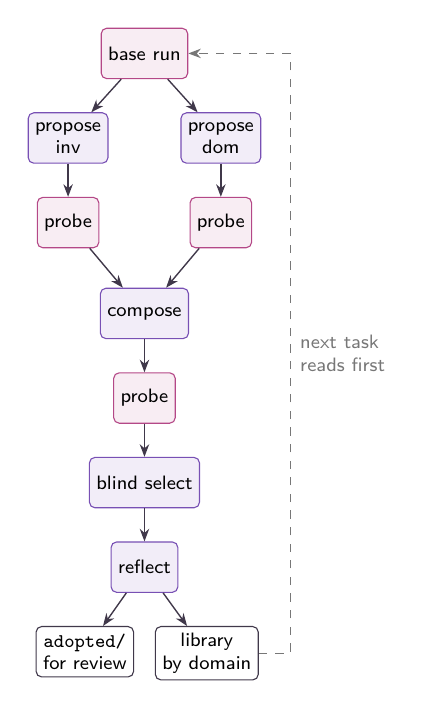
\begin{tikzpicture}[
  font=\sffamily\scriptsize,
  node distance=4.2mm and 3mm,
  run/.style={draw=acpink, fill=acpink!10, rounded corners=2pt, align=center, minimum height=6.4mm, inner sep=2.5pt},
  ask/.style={draw=acpurple, fill=acpurple!10, rounded corners=2pt, align=center, minimum height=6.4mm, inner sep=2.5pt},
  res/.style={draw=acdark, fill=white, rounded corners=2pt, align=center, minimum height=6.4mm, inner sep=2.5pt},
  arr/.style={-{Stealth[length=1.6mm]}, draw=acdark, line width=0.5pt}]
\node[run] (base) {base run};
\node[ask, below left=of base, xshift=4mm] (inv) {propose\\inv};
\node[ask, below right=of base, xshift=-4mm] (dom) {propose\\dom};
\node[run, below=of inv] (pinv) {probe};
\node[run, below=of dom] (pdom) {probe};
\coordinate (mid) at (pinv.south -| base);
\node[ask, below=5mm of mid] (comp) {compose};
\node[run, below=of comp] (pcomp) {probe};
\node[ask, below=of pcomp] (sel) {blind select};
\node[ask, below=of sel] (refl) {reflect};
\node[res, below left=of refl, xshift=6mm] (adopt) {\code{adopted/}\\for review};
\node[res, below right=of refl, xshift=-6mm] (lib) {library\\by domain};
\draw[arr] (base) -- (inv); \draw[arr] (base) -- (dom);
\draw[arr] (inv) -- (pinv); \draw[arr] (dom) -- (pdom);
\draw[arr] (pinv) -- (comp); \draw[arr] (pdom) -- (comp);
\draw[arr] (comp) -- (pcomp); \draw[arr] (pcomp) -- (sel);
\draw[arr] (sel) -- (refl); \draw[arr] (refl) -- (adopt); \draw[arr] (refl) -- (lib);
\draw[arr, dashed, draw=acgray] (lib.east) -- ++(4mm,0) |- node[pos=0.25, right, align=left, text=acgray] {next task\\reads first} (base.east);
\end{tikzpicture}
\caption{One round of \code{refine}. Pink stages run the task through
\code{ac run}; purple stages are Claude sessions reading evidence served as
files. A candidate identical to an earlier harness reuses its run.}
\label{fig:round}
\end{figure}

\section{Evaluation}
\label{sec:eval}

We ran the three interaction tasks --- a poke-able jelly, finger-painted
trails that fade, a playable snake --- through three batches: a first round on
jelly alone (R0), all three with the hosted default model, DeepSeek~V4.1~Flash
(R1), and all three with Claude Sonnet~5.5 writing the pieces (R2). Claude
Sonnet~5 was the improver throughout. Table~\ref{tab:rounds} gives every run.

\begin{table*}[t]
\centering
\small
\begin{tabular}{@{}llllllr@{}}
\toprule
Batch & Task & Base & inv & dom & Chosen & Claude \\
\midrule
R0 Flash & jelly & \yes{} 69\,s / 6 rounds & $\times$ output limit & \yes{} 77\,s / 4 & base & \$1.40 \\
R1 Flash & jelly & \yes{} 77\,s / 4 & $\times$ output limit & \yes{} 85\,s / 5 & \textbf{dom} & \$1.33 \\
R1 Flash & trails & \yes{} 75\,s / 12 & \yes{} 69\,s / 11 & \yes{} 76\,s / 8 & base & \$2.12 \\
R1 Flash & snake & \yes{} 19\,s / 4 & \yes{} 23\,s / 4 & \yes{} 31\,s / 5 & \textbf{dom} & \$2.39 \\
R2 Sonnet 5.5 & jelly & \yes{} 39\,s / 3 & \yes{} 32\,s / 3 & \yes{} 33\,s / 3 & base & \$1.91 \\
R2 Sonnet 5.5 & trails & \yes{} 24\,s / 2 & \yes{} 25\,s / 2 & = base & \textbf{inv} & \$1.62 \\
R2 Sonnet 5.5 & snake & $\times$ out of allowance & --- & --- & --- & \$0.73 \\
\bottomrule
\end{tabular}
\caption{Every run, one per arm. A tick is a delivered turn, with wall time and
model rounds; \emph{output limit} means the model's 8,192-token response cap
ended the turn before a save. The composed candidate equalled one of the others
in every round except R1 trails, where it also delivered (67\,s / 10) and was
not chosen. Claude is the improvers' cost per task. R2 snake failed before
reaching the model and is excluded from every claim below.}
\label{tab:rounds}
\end{table*}

\begin{figure*}[t]
\centering
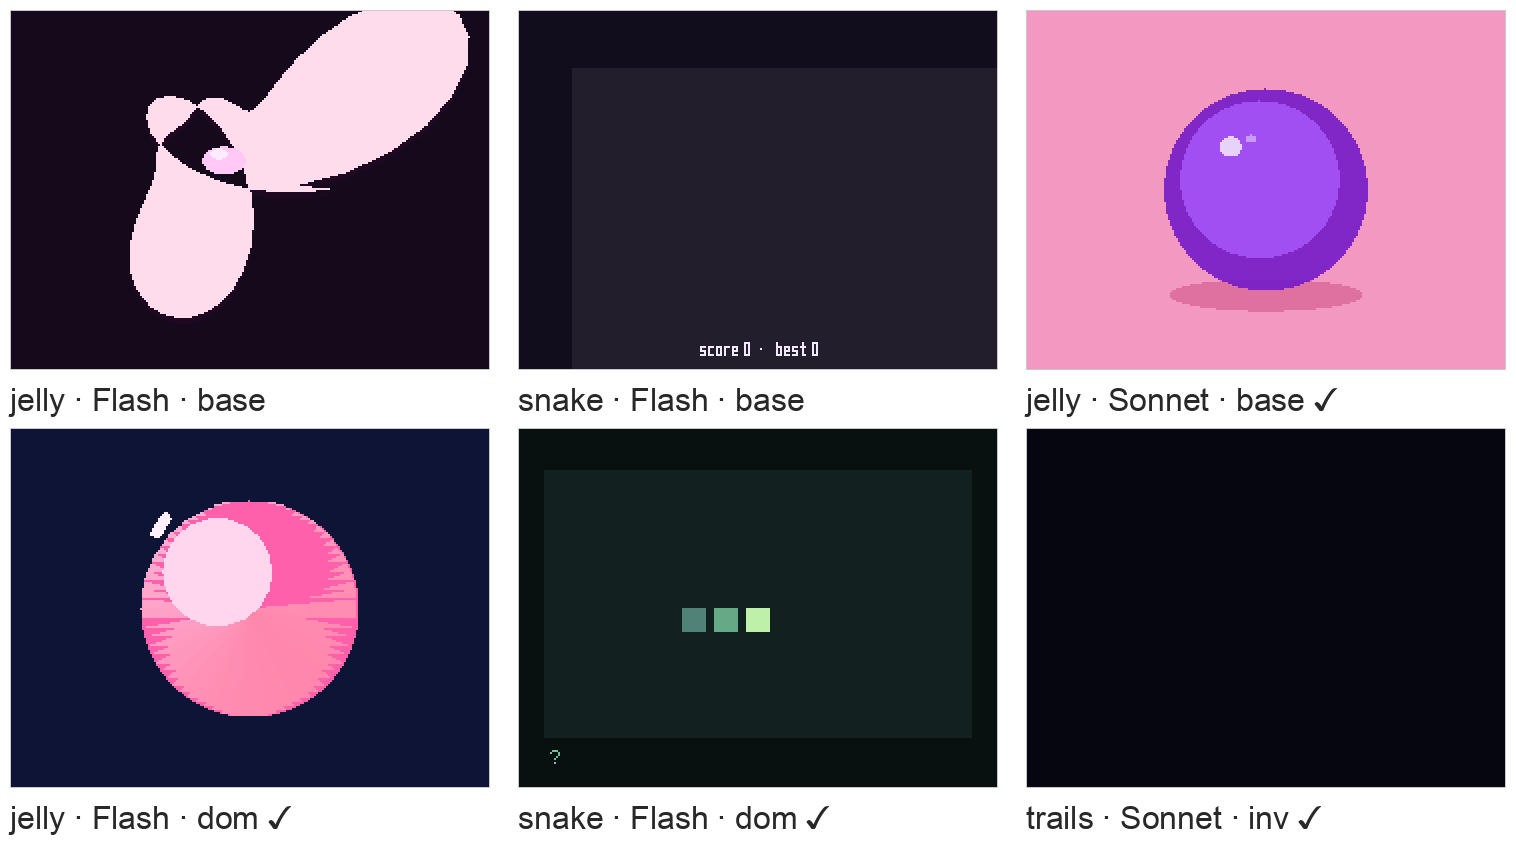
\includegraphics[width=0.92\textwidth]{frames}
\caption{The last frame \code{ac check} recorded for six runs; a tick marks the chosen piece. Left: the R1
jelly base folds into lobes under a poke where the adopted candidate dents and
holds. Middle: the R1 snake base reaches game over before any input; the
adopted candidate waits. Right: Sonnet~5.5's jelly base, chosen over both
candidates, and its chosen trails piece, blank because the frame was taken
after the trail faded --- the case its adopted rule names.}
\label{fig:frames}
\end{figure*}



\subsection{What the rounds found}
\textbf{Rules that changed the piece.} In R1 jelly the base piece's spring rim
folded through itself under a poke; the dom editor added to
\code{piece-visual} a rule bounding impulse against stiffness, clamping rim
points away from the centre, and judging over several frames, and its piece
dented and settled (Figure~\ref{fig:frames}). In R1 snake the base game had
already ended before the check's first input --- an empty board reading
\emph{score 0}; the adopted rule holds a self-moving game in a ready state
until the player's first key or touch. In R2 trails the inv editor added to
\code{piece-reply} that the model must say when its check exercised a different
interaction from the one it describes --- a tap standing in for a drag, a frame
taken after a fade --- and that piece was chosen.

\textbf{A rule that helped and was not adopted.} In R0 the base run lost two
rounds to \code{circle} and \code{screen} used in functions that had not
destructured them. The dom edit to \code{api-workflow} --- each lifecycle
function receives its own copy of the API --- gave a clean first save, and the
reflector marked it \emph{helped}. The selector still preferred the base piece,
which wobbled on a plain tap. Selection judges pieces, not edits; the library
is where such an edit survives, as a medium-confidence lesson.

\textbf{A failure that was evidence.} The inv candidate on jelly hit the output
cap in R0 and again in R1. In both, the third response spent most of its 8,192
tokens thinking --- 6,379 in R1 --- before a save could fit. Both inv edits had
added a check-before-saving \emph{procedure}. We read this as the edit hurting
on a reasoning model, not noise: state the fact, not a routine to run.

\textbf{A model that needed little help.} Every Sonnet~5.5 run delivered in two
or three rounds and 24--39\,s, against 4--12 rounds and 19--100\,s for Flash.
Its editors proposed the same kinds of rule; with Sonnet writing, only the
reporting rule changed which piece won.



\section{What the method needed here}
\label{sec:lessons}

Two changes to the loop came from its own output. In R0 the inv editor wrote
its rule into a section only terminal sessions in a repository receive, so its
probe could not test it. Runs now record the system prompt they sent, match it
against every section's fixed text, and give editors the list; in R1 and R2
every edit landed in a section the run received. And R2 snake ran out of the
day's inference allowance before reaching the model, yet the improvers were
paid \$0.73 to read the failure; a base run that never reaches the model now
stops the batch.

A third came from the session itself. The plan was being carried out by two
agent sessions at once, and they implemented the same step twice before one
noticed. The record in the repository is now the first thing a session reads.

\section{Limitations and ethics}
\label{sec:limits}

\textbf{One run per arm.} Every comparison above is a single base run against a
single candidate run, and Flash is noisy: R0 and R1 ran the same base harness on
jelly and took six and four rounds. A finding here is a reason to look, not a
measured effect. An earlier hand-run pass on Whistlegraph targets, with
pixel-scored re-renders, reached the same conclusion: a loop needs several runs
per arm and, where possible, a scorer per task.

\textbf{The verdict is narrow.} \emph{Delivered} means the final source ran for
four seconds, under one tap and one space, without an error. It does not
establish that a game is playable or a trail visible; the blank frame in
Figure~\ref{fig:frames} is a delivered run. The selector and reflector are
models judging models, and the same model family edits and judges.

\textbf{Always-on cost.} Two adopted rules are specific to a kind of piece ---
spring rims, self-moving games --- but were written into \code{piece-visual},
which every piece request carries. They should not ship there as written.

\textbf{Cost and consent.} The seven rounds cost \$11.50 of Claude usage and
the day's \ac{} inference allowance. No person's work or data was used: tasks
are synthetic requests and pieces were never published. Requests went to the
inference vendors as in ordinary use; transcripts and frames are stored only on
the machine that ran them.

\section{Conclusion}
\label{sec:conclusion}

Moving the prompt into named sections was the step everything else waited on,
and it was the cheap one. With the harness editable and every embedding
reading it, a round costs a few dollars and leaves a diff a person can read.
The first rounds found real failure modes --- a folding rim, a game lost before
it began, an unchecked claim --- and one rule that helped but lost the vote.
They also found that the stronger model needed the harness least. Whether these
rules hold is a question for repeated runs, which is the next thing to build.

\balance
\bibliographystyle{plainnat}
\bibliography{references}

\end{document}
